\chapter{Resultados}

Este capítulo muestra los resultados obtenidos en cada fase de la metodología de esta investigación.

\section{Comprensión del problema y preparación de los datos}

En la fase de comprensión del problema se obtuvo  un marco teórico referente a todas las técnicas utilizadas en esta investigación para tratar con documentos textuales no estructurados.
En la fase de  preparación de los datos se obtuvo un corpus limpio compuesto por 10.000 documentos.

\section{Modelado}

En esta fase se obtuvieron modelos para estructurar los documentos y modelos de aprendizaje supervisado y no supervisado para identificar áreas de conocimiento en los trabajos de grado .

\textbf{Modelos para estructurar el corpus}

La tabla \ref{tab:ProgramasDM} muestra el estadístico de Hopkins para cada conjunto de datos generado. 


\begin{table}[H]\centering
	\caption{Descripción de la tendencia al agrupamiento en los conjuntos de datos.}\label{tab:ProgramasDM}
	\begin{tabularx}{\textwidth}{XXXm{6.0cm}}\toprule

Modelo &  \multicolumn{1}{c}{Estadístico Hopkins} & \multicolumn{1}{c}{Descripción} \\ 
Bow & 0.61 & Modelo Bow generando un conjunto de datos de 10.000 filas * 20.000 
columnas usando unigramas y bigramas.
Este método descarta términos que aparezcan en más del 70\% de documentos.  \\ 
Bow &  0.58 & Modelo Bow generando un conjunto de datos de 10.000 filas * 10.000 
columnas usando unigramas y bigramas.
Este método descarta términos que aparezcan en más del 70\% de documentos.   \\ 
Tf-idf & 0.54 & Modelo Tf-id generando un conjunto de datos de 10.000 filas * 20.000 
columnas usando unigramas y bigramas.
Este método descarta términos que aparezcan en más del 70\% de documentos.  \\ 
Tf-idf &  0.52 & Modelo Tf-id generando un conjunto de datos de 10.000 filas * 10.000 
columnas usando unigramas y bigramas.
Este método descarta términos que aparezcan en más del 70\% de documentos.   \\ 
Doc2vec & 0.38 & Este método representa un documento mediante 
un vector de tamaño 20
usando el algoritmo bolsa de palabras distribuida  (PV-DBOW)   \\ 
Doc2vec & 0.42  & Este método representa un documento mediante
un vector de tamaño 20
usando el algoritmo memoria distribuida (PV-DM) \\  \bottomrule
	\end{tabularx}

\end{table}

Con un umbral establecido en 0.5 podemos confirmar que existe tendencia al agrupamiento en los conjuntos de datos generados por los modelos Doc2vec bolsa de palabras distribuida (PV-DBOW) y Doc2vec memoria distribuida (PV-DM).
%Los resultados muestran una mejor tendencia al agrupamiento en los modelos Doc2vec,
Los modelos Doc2vec  logran captar relaciones conceptuales mediante el contexto que representa cada documento, usando esta representación se podrá medir qué tan relacionado está un documento con respecto a los demás.	

%%%%%%%%%%%%%%%%%%%%%%%%%%%%%%%%%%%%%%%%%%%%%%%%%%%%%%%%%%%%
\textbf{Modelos de aprendizaje automático  }

Con el fin de descubrir grupos de conocimiento de acuerdo al contexto de los diferentes trabajos de grado se corrió el algoritmo k-medias.

Para la selección del k óptimo generamos diferentes grupos iterando k desde 20 a 44 evaluando el coeficiente de Silhouette y el error cuadrático en los 2 conjuntos de datos generados con el modelo Doc2vec ya que tienen tendencia al agrupamiento.


\begin{figure}[H]
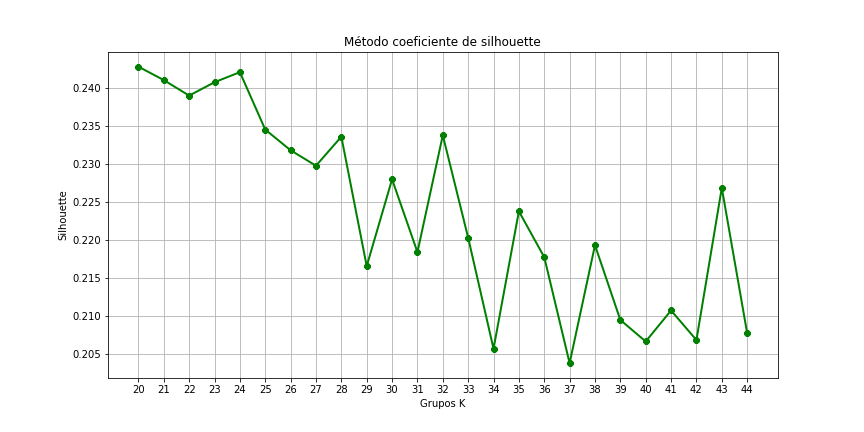
\includegraphics[width=1\textwidth]{Silhouette}
\caption{Método coeficiente de Silhouette algoritmo Kmedias }
\label{fig:proceso3}
\end{figure}

\begin{figure}[H]
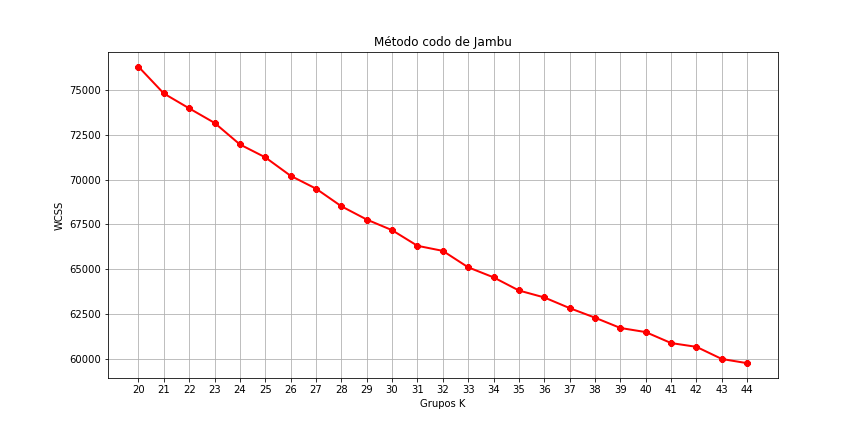
\includegraphics[width=1\textwidth]{WCSS}
\caption{Método de codo de Jambu algoritmo Kmedias}
\label{fig:proceso4}
\end{figure}

En la figura  \ref{fig:proceso3} se visualiza el método de coeficiente de Silhouette; el cual sugiere que el número adecuado de grupos es de 24, en la figura  \ref{fig:proceso4} se visualiza el método del codo de Jambu; 
para el cual miramos que a medida que k se incrementa la distancia de los puntos al centroide va disminuyendo. Para la selección del K óptimo  se contrasto los dos métodos y se eligió el k en 32; ya que miramos que su coeficiente de Silhouette está entre los más altos y a la vez la distancia de los puntos al centroide es baja. Por lo tanto se corrió el algoritmo k medias con k =32, con el fin de clasificar los documentos en 32 áreas de conocimiento de acuerdo a su temática de contexto. Para clasificar futuros trabajos de grado en los grupos encontrados se entrenó modelos de aprendizaje supervisado; los cuales se verán en el capítulo de discusión.



%%%%%%%%%%%%%%%%%%%%%%%%%%%%%%%%%%%%%%%%%%%%%%%%%%%%%%%%%%%%%%%%%

\section{Implementación}


Maskana está compuesta por 3 módulos: el módulo GUI, el módulo núcleo y el módulo de conexión. En esta fase se presenta el cuarto módulo denominado servicios de minería de texto, el cual se puede observar en la figura \ref{fig:implementacion1}.


\begin{figure}[H]
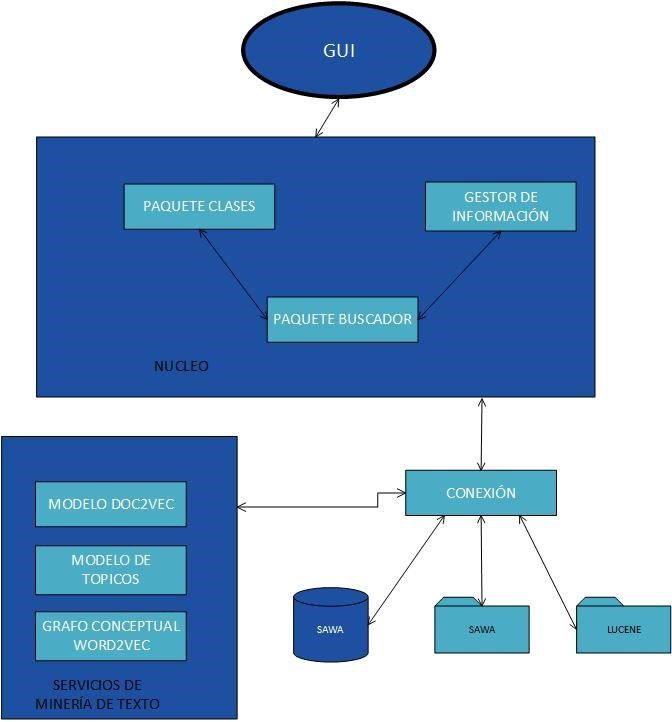
\includegraphics[width=0.9\textwidth]{implementacion1.png}
\caption{Arquitectura de Maskana.}
\label{fig:implementacion1}
\end{figure}

\textbf{Módulo de Servicios de Minería de texto.}

Este módulo es el encargado de brindar servicios web que conectan a Maskana con los modelos elaborados en la sección de modelado, en este módulo
 se encuentran los algoritmos para relacionar documentos conceptualmente,
 conocer los temas o tópicos principales de los trabajos de grado consultados y sus relaciones.
 A continuación, se hace una descripción de los submódulos que lo componen.

\textbf{Modelo Doc2vec:}
Este submódulo lleva el nombre del modelo Doc2vec,el cual se encarga de realizar la representación vectorial de todos los documentos del repositorio, generando vectores conceptuales teniendo en cuenta el contexto de los documentos con los que fue entrenado, estos vectores están almacenados en la base de datos Sawa mediante el módulo de conexión, 
se implementó el algoritmo \ref{alg:maskanita1} , el cual permite  encontrar similitudes conceptuales entre los documentos del repositorio; ayudando a extender las búsquedas que realizan los usuarios de la herramienta Maskana.

\begin{algorithm}
    \renewcommand{\algorithmicrequire}{\textbf{Input:}}
    \renewcommand{\algorithmicrequire}{\textbf{Input:}}
    \renewcommand{\algorithmicensure}{\textbf{Output:}}
    \renewcommand{\algorithmicprint}{\textbf{break}}
  \caption{ Maskanita recomendación de trabajos de grado.}
  \label{alg:maskanita1}
  \algsetup{indent=2em}
  \footnotesize
  \begin{algorithmic}[1]
\REQUIRE {D: documento resultado de búsqueda} 
\REQUIRE {Corpus\_doc2vec : corpus estructurados con el modelo doc2veca} 
\ENSURE {DocRel: conjunto de documentos relacionados a D}
\STATE $DocRel \leftarrow \emptyset$
\STATE vector\_documento=doc2vec(D)
\STATE grupo\_documento=xgboost.clasificar(vector\_documento)
\FOR {each doc  \in$ Corpus\_doc2vec  \in$  grupo\_documento }
	\IF{ similitud\_coseno( vector\_documento,doc2vec(doc))>0.7}
		  \STATE {DocRel $\leftarrow $adicionar(DocRel,doc) }
		% \STATE {D $\leftarrow$ points $\in c$ }
	\ENDIF
\ENDFOR
\STATE {ordenar(DocRel) }
\end{algorithmic}
\end{algorithm}

El algoritmo \ref{alg:maskanita1} implementado en Maskana permite realizar búsquedas temáticas y recomendaciones de trabajos relacionados contextualmente con otros. 
Como entrada se envía la consulta o un documento del repositorio,
el modelo Doc2vec se encarga de realizar la representación vectorial de la entrada,
el modelo Xgboost se encarga de clasificar el vector generado en los dominios o grupos encontrados; para filtrar el resultado al dominio clasificado y obtener los documentos que tengan  mayor similitud conseno.


%\begin{figure}[H]
%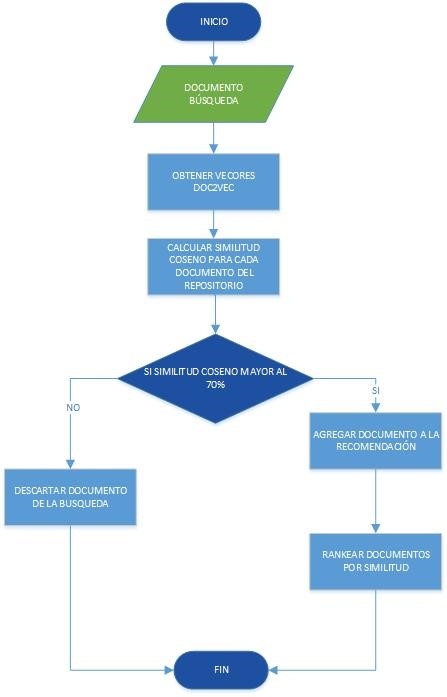
\includegraphics[width=0.7\textwidth]{implementacion2}
%\caption{Diagrama de flujo algoritmo Maskanita recomendación de trabajos de grado.}
%\label{fig:implementacion2}
%\end{figure}

\textbf{Modelo de tópicos:} En este submódulo se encuentra implementado el algoritmo LDA para conocer los diferentes tópicos 
o temas relacionados con los trabajos de grado, recomendados por el algoritmo Maskanita. Como primer paso se toma los documentos recomendados por el algoritmo Maskanita, como segundo paso 
se obtiene el número de temas a calcular por parte del usuario, seguidamente se ejecuta el algoritmo LDA de la librería Gensim de Python, 
Finalmente se obtienen los temas principales que componen los documentos recomendados y se los visualiza mediante el servicio web de este submódulo.

\begin{figure}[H]
\centering
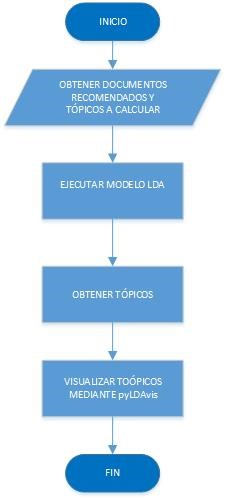
\includegraphics[width=0.3\textwidth]{implementacion3}
\caption{Proceso submódulo modelo de tópicos.}
\label{fig:implementacion3}
\end{figure}


\textbf{Grafo conceptual Word2vec:} En este submódulo se encuentra implementado  el algoritmo \ref{alg:maskanita2}, útil para representar relaciones conceptuales del contenido de los trabajos de grado recomendados por el algoritmo Maskanita  \ref{alg:maskanita1}. 
El primer paso toma como entrada los documentos recomendados por Maskanita \ref{alg:maskanita1}, En segundo lugar, se obtiene conceptos relevantes de los documentos de entrada mediante la tarea de reconocimiento de entidades nombradas de la librería Spacy de Python,
Para cada entidad o concepto reconocido se aplica el modelo Word2vec para conocer sus relaciones, finalmente se construye el grafo conceptual usando la librería D3.js y  el servicio web implementado en este submódulo.  


\begin{algorithm}[H]
    \renewcommand{\algorithmicrequire}{\textbf{Input:}}
    \renewcommand{\algorithmicensure}{\textbf{Output:}}
    \renewcommand{\algorithmicprint}{\textbf{break}}
  \caption{ Maskanita relaciones conceptuales de trabajos de grado.}
  \label{alg:maskanita2}
  \algsetup{indent=2em}
  \footnotesize
  \begin{algorithmic}[1]
\REQUIRE {T: contenido textual documentos relacionados } 
\ENSURE {G: Grafo Conceptual }
\STATE $conceptos\_ner \leftarrow \emptyset$
\STATE $G \leftarrow \emptyset$
\STATE {spacy.load('es\_core\_news\_sm') }
\FOR {each token  \in$ T }
	\IF{spacy.isNer(token)}
		  \STATE {$conceptos\_ner $\leftarrow $adicionar(conceptos\_ner,token)}
		% \STATE {D $\leftarrow$ points $\in c$ }
	\ENDIF
\ENDFOR

\FOR {each c  \in$ conceptos\_ner }
	\FOR {rl  \in$  word2vec.sim(c) }
		  \STATE {$n1 $\leftarrow $crearNodo(c)}
		  \STATE {$n2 $\leftarrow $crearNodo(rl)}
		  \STATE {$G $\leftarrow $relacionarNodos(n1,n2)}
	\ENDFOR
\ENDFOR


\end{algorithmic}
\end{algorithm}


%%%%%%%%%%%%%%%%%%%%%%%%%%%%%%%%%%%%%%%%%%%%%%%%%%%%%%%%%%%%%%%%%%



\textbf{Interpretación de las categorías  mediante grafos conceptuales.}

%En esta sección se interpreta el conocimiento obtenido mediante grafos conceptuales, los cuales permiten visualizar relaciones conceptuales temáticas; organizando contextualmente el corpus de trabajos de grado; soportadas por el modelo Word2vec, estos fueron elaborados para trabajos de grado relacionados encontrados en diferentes áreas de conocimiento de cada grupo formado.
%En la figura \ref{fig:procesocinco} se observa la distribución de los diferentes documentos del repositorio; estructurados por el modelo Doc2vec con su respectivo grupo en coordenadas de las componentes principales. A continuación, se interpreta cada grupo y los dominios de conocimiento que representan.

En este apartado se  se interpreta el conocimiento obtenido en cada grupo de conocimiento encontrado mediante grafos conceptuales creados por el algoritmo \ref{alg:maskanita2},
el cual permite visualizar relaciones conceptuales temáticas;

En la figura \ref{fig:procesocinco} se observa la distribución de los diferentes documentos del repositorio; estructurados por el modelo Doc2vec con su respectivo grupo en coordenadas de las componentes principales.


\begin{figure}[H]
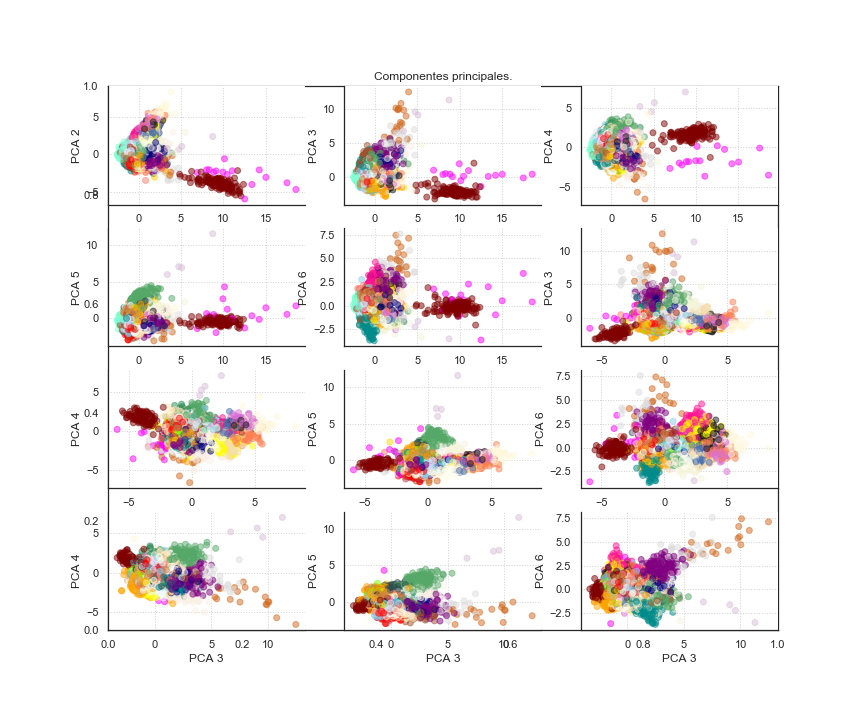
\includegraphics[width=1\textwidth]{proceso5}
\caption{Biplot componentes principales}
\label{fig:procesocinco}
\end{figure}


\begin{table}[H]\centering
\caption{Resumen grupos}\label{tab:tablaeg}
	\begin{tabularx}{\textwidth}{XXXm{3.0cm}}\toprule

Grupo &  \multicolumn{1}{c}{Cantidad } \\ 
0&      309\\
1&     382\\
2&     346\\
3&    409\\
4&   137\\
5&   175\\
6&   159\\
7&   456\\
8&   341\\
9&   389\\
10& 30\\
11& 158\\
12& 510\\
13& 237\\
14& 317\\
15& 206\\
16& 230\\
17& 145\\
18& 137\\
19& 353\\
20& 282\\
21& 126\\
22& 344\\
23& 68\\
24& 226\\
25& 192\\
26& 87\\
27& 374\\
28& 326\\
29& 233\\
30& 211\\
31& 181\\


 \bottomrule
	\end{tabularx}
	
\end{table}

 La tabla  \ref{tab:tablaeg}  indica cuántos trabajos quedaron en cada cluster, a continuación, se interpreta cada grupo y los dominios de conocimiento que representan.

En el grupo 0 se encuentran trabajos relacionados a temáticas respectivas a los derechos humanos, derechos constitucionales, derechos laborales, derechos penales, derecho judicial, derecho administrativo, leyes y artículos constitucionales.

En el grupo 1 se encuentran trabajos de grado relacionados a temáticas de desempleo, desigualdad social , condiciones socioeconómicas, fortalecimiento del comercio y economía. 

En el grupo 2 se encuentran trabajos relacionados a temáticas de relaciones interfamiliares, estudios de violencia, conflictos familiares, machismo, patriarcado y problemáticas dentro del contexto sociológico como describe la figura \ref{fig:grupo14}.
\begin{figure}[H]\centering
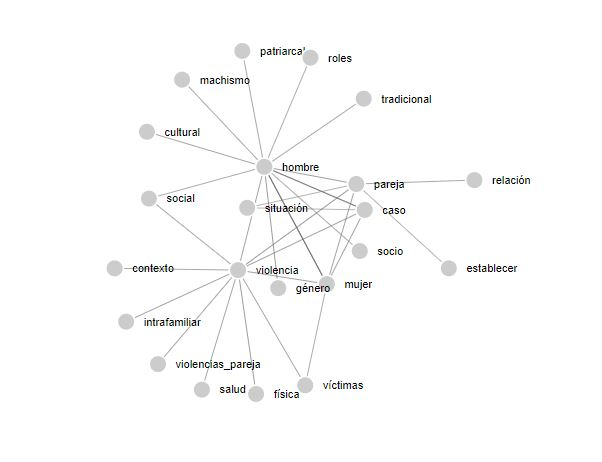
\includegraphics[width=0.8\textwidth]{grupo14}
%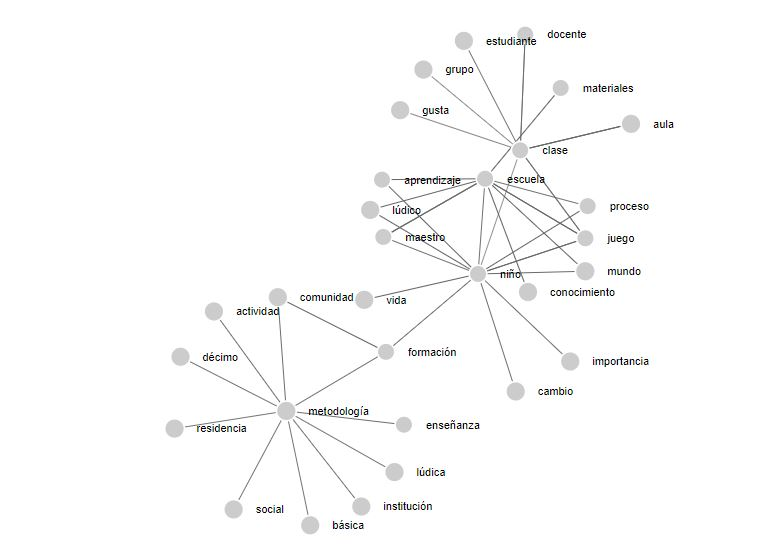
\includegraphics[width=0.8\textwidth]{grupo8}
\caption{Grafo  relaciones temáticas grupo 2 }
\label{fig:grupo14}
\end{figure}

%En el grupo 8 se encuentran trabajos relacionados con temáticas pedagógicas para la educación básica primaria. 
%\begin{figure}[H]\centering
%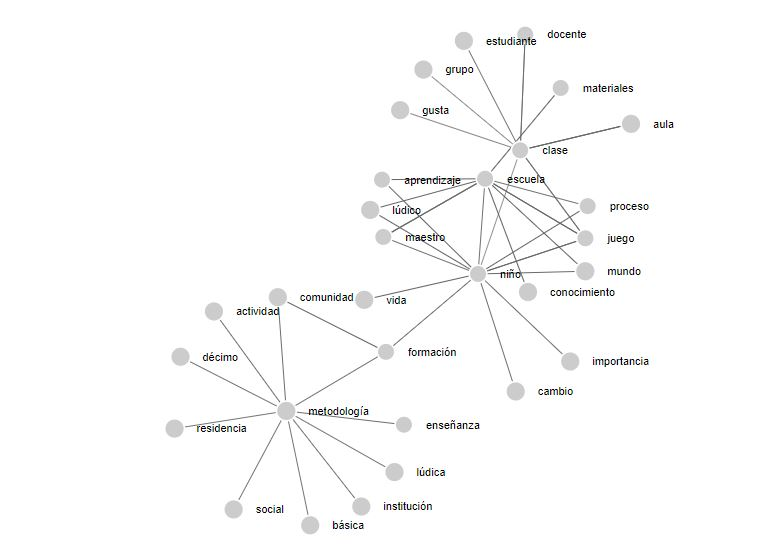
\includegraphics[width=0.8\textwidth]{grupo8}
%\caption{Grafo  relaciones temáticas  grupo 8 }
%\label{fig:grupo8}
%\end{figure}

%En la figura \ref{fig:grupo14} podemos observar relaciones contextuales complementarias del grupo 8 tales como: escuela, maestros , aulas de clase, estrategias y metodologías didácticas de aprendizaje basadas en lúdicas y juegos para niños estudiantes de básica  primaria.

En el grupo 3 se encuentran trabajos de grado relacionados a temáticas de planeación estratégica empresarial, marketing y estudios de comercio en  organizaciones, como se puede observar en la figura \ref{fig:grupo5} .
\begin{figure}[H]\centering
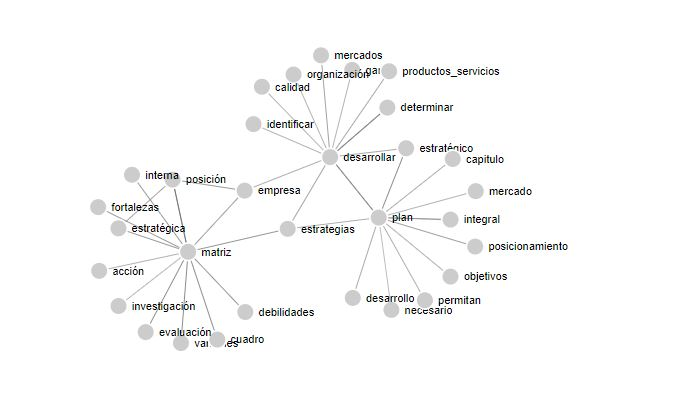
\includegraphics[width=1\textwidth]{grupo5}
\caption{Grafo relaciones temáticas grupo 3 }
\label{fig:grupo5}
\end{figure}

En el grupo 4 se encuentran trabajos de grado relacionados al departamento de idiomas, todos los documentos de este grupo se encuentran en idioma inglés, reprentado en la figura \ref{fig:grupo6}.

\begin{figure}[H]\centering
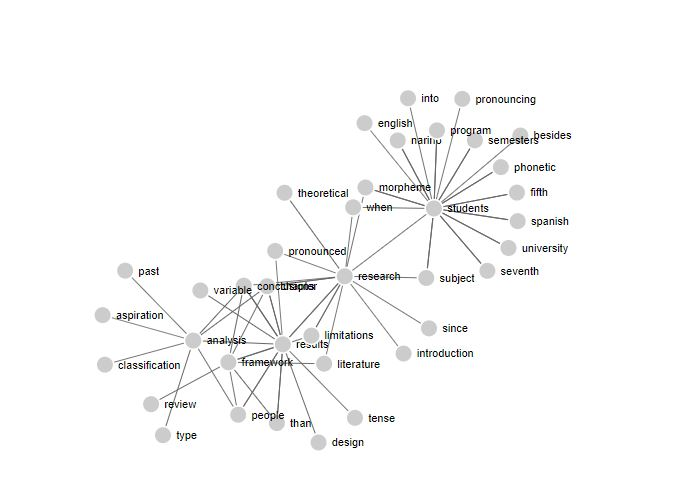
\includegraphics[width=0.8\textwidth]{grupo6}
\caption{Grafo  relaciones temáticas grupo 4 }
\label{fig:grupo6}
\end{figure}

En el grupo 5 se encuentran trabajos de grados vinculados a la facultad de ciencias exactas, específicamente al programa de Biología, evaluando diferentes tratamientos para encontrar diferencias estadísticamente significativas entre estos y así mejorar el crecimiento y producción de especies. %%

En el grupo 6 se encuentran trabajos relacionados al estudio de modelamiento de fluidos.

En el grupo 7 se encuentran trabajos de grado relacionados a temas de cultura, carnavales, historia y desarrollo social.
\begin{figure}[H]\centering
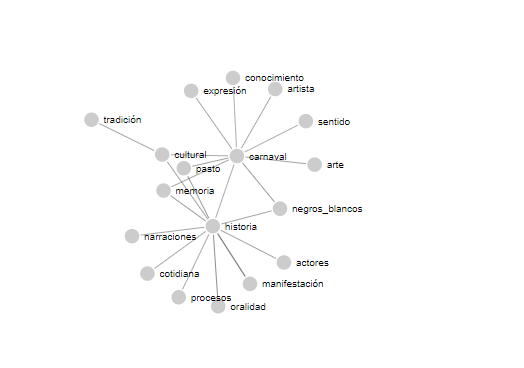
\includegraphics[width=0.8\textwidth]{grafocul0}
\caption{Grafo  relaciones temáticas grupo 7 }
\label{fig:grafoculcero}
\end{figure}



La figuera \ref{fig:grafoculcero}  se muestra el grafo  conceptual  de los trabajos de grado clasificados en el grupo 7, donde se observa conceptos relacionados referentes al carnaval de negros y blancos, cultura, artes , maestros y artesanos.

En el grupo 8 se encuentran trabajos relacionados a construcción, desarrollo, gestión de calidad y auditoría de obras civiles.

En el grupo 9 se encuentran trabajos de grado relacionados con temáticas pedagógicas de aprendizaje   y estrategias lúdicas de aprendizaje  para estudiantes.

En el grupo 10 se encuentran trabajos de grado relacionados específicamente a ingeniería de software, lenguaje unificado de modelado UML, desarrollo y construcción de módulos y sistemas de información a la medida.

En el grupo 11 se encuentran trabajos relacionados a telemática, microcontroladores, reconocimiento de imágenes, redes neuronales ,  espectro electromagnético,  series temporales,  aplicaciones en vulcanología y sismología. 

En el grupo 12 se encuentran trabajos de grado vinculados al programa de ingeniería agroindustrial referentes a temáticas de desarrollo, comercialización, industrialización, estudios de oferta y demanda de productos agropecuarios.

En el grupo 13 se encuentran trabajos de grado en temáticas de ordenamiento territorial, desarrollo sostenible y seguridad social.  %%%%%

En el grupo 14 se encuentran trabajos de grado relacionados con proyectos referentes a entornos y herramientas virtuales de aprendizaje.

En el grupo 15 se encuentran trabajos de grado vinculados a esquemas de seguridad, salud ocupacional en la industria y riesgos laborales como se describe en la figura \ref{fig:grupo22}


\begin{figure}[H]\centering
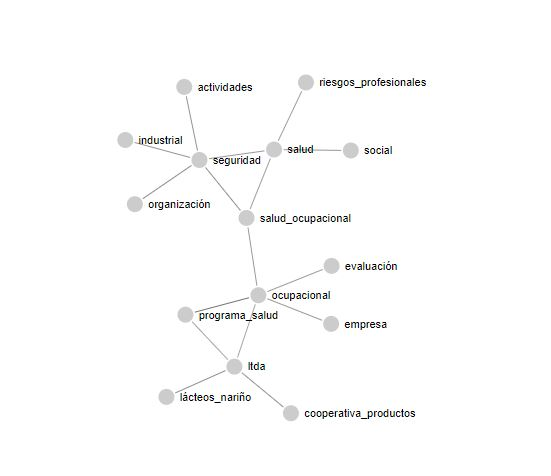
\includegraphics[width=0.8\textwidth]{grupo22}
\caption{Grafo  relaciones temáticas grupo 15}
\label{fig:grupo22}
\end{figure}


En el grupo 16 se encuentran trabajos de grado relacionados a cultivos, recursos hídricos  , plantas, especies y temáticas agroforestales como se observa en la figura \ref{fig:grupo1especies}.
\begin{figure}[H]\centering
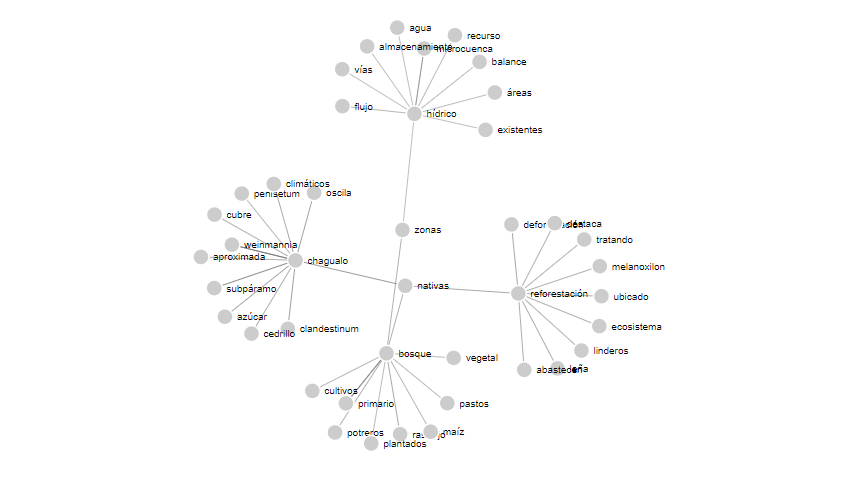
\includegraphics[width=1\textwidth]{grupo1especies}
\caption{Grafo relaciones temáticas grupo 16 }
\label{fig:grupo1especies}
\end{figure}

El grupo 17 contiene tópicos relacionados con bacterias, microorganismos, compuestos antioxidantes, proteínas y aminoácidos como se describe en la figura \ref{fig:grupo25}.
\begin{figure}[H]\centering
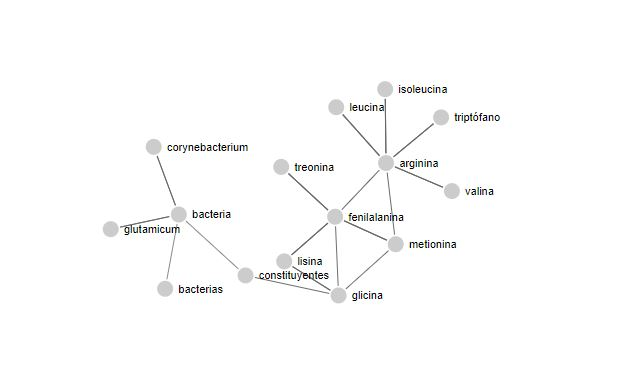
\includegraphics[width=0.8\textwidth]{grupo25}
\caption{Grafo  relaciones temáticas grupo 17}
\label{fig:grupo25}
\end{figure}

En el grupo 18 se encuentran trabajos relacionados con temáticas temáticas afines a administración, economía y finanza empresarial.

En el grupo 19 se encuentran trabajos relacionados a temáticas sociales, desarrollo humano sostenible, desarrollo económico social, derecho internacional humanitario y políticas comunitarias.

En el grupo 20 se encuentran trabajos de grado de la facultad de artes, referentes a temáticas culturales, artesanías e  historia del arte.

En el grupo 21 se encuentran trabajos relacionados a la facultad de ciencias económicas y administrativas los cuales involucran temáticas de comercio exterior, aduanas, exportaciones, impuestos, empresas, fiscalización y estudios de mercados.


En el grupo 22 se encuentran trabajos de grado relacionados con planes de ordenamiento  territorial   y ecoturismo tal como se observa en la figura \ref{fig:ordenaminetoimg}.


\begin{figure}[H]\centering
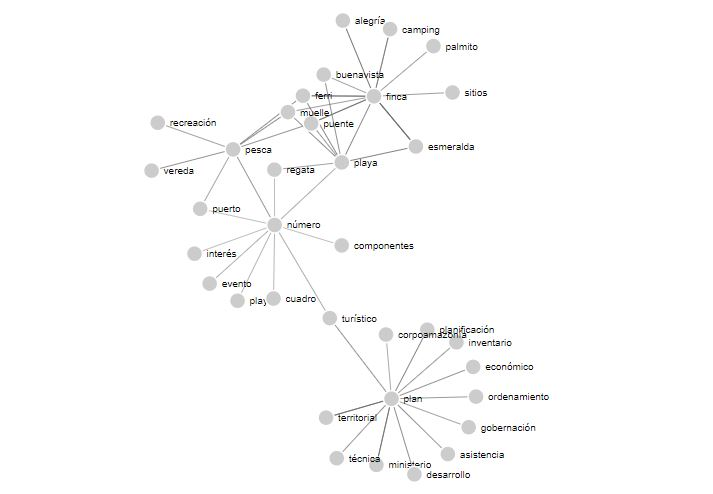
\includegraphics[width=1\textwidth]{ordenaminetoimg}
\caption{Grafo relaciones temáticas grupo 22 }
\label{fig:ordenaminetoimg}
\end{figure}

En el grupo 23 se encuentran trabajos de grado de la facultad de ciencias agrícolas, específicamente del programa de ingeniería agronómica, relacionando temáticas referentes a estudios de variedades de especies de granos, tubérculos, plantas y técnicas de comparación de diferentes tratamientos agronómicos mediante pruebas de Tukey y validaciones estadísticas
como se representa en la figura \ref{fig:grupo25}.
\begin{figure}[H]\centering
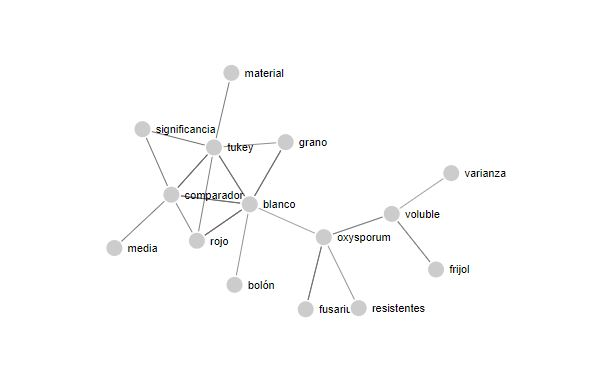
\includegraphics[width=0.8\textwidth]{grupo28}
\caption{Grafo  relaciones temáticas grupo 23}
\label{fig:grupo25}
\end{figure}


En el grupo 24 se encuentran trabajos relacionados con medicina veterinaria, en la figura \ref{fig:grupo7} se aprecia relaciones entre enfermedades causadas por las bacterias babesia y  anaplasma en equinos.

\begin{figure}[H]\centering
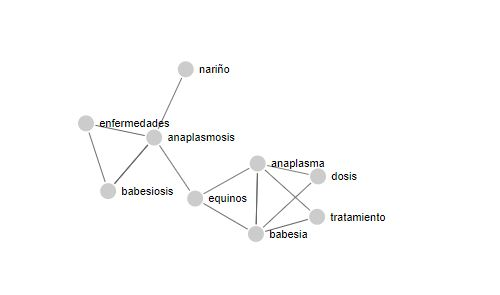
\includegraphics[width=0.8\textwidth]{grupo7}
\caption{Grafo  relaciones temáticas grupo 24 }
\label{fig:grupo7}
\end{figure}

En el grupo 25 se encuentran trabajos de grado relacionados con proyectos de priorización de áreas ambientales, caracterización de sistemas agroforestales, investigación de especies y reservas naturales.  %%

En el grupo 26 se encuentran trabajos de grado relacionados con música.

En el grupo 27 se encuentran trabajos relacionados con temáticas pedagógicas para la educación. 
\begin{figure}[H]\centering
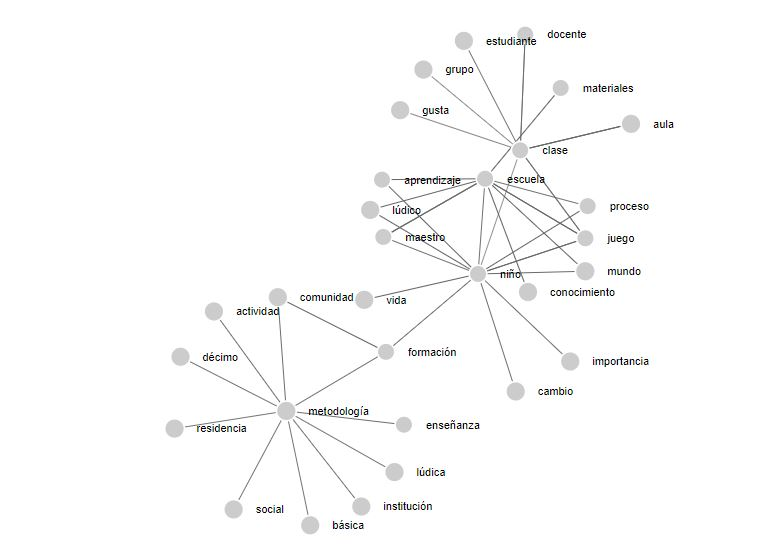
\includegraphics[width=0.8\textwidth]{grupo8}
\caption{Grafo  relaciones temáticas grupo 27 }
\label{fig:grupo8}
\end{figure}

En la figura \ref{fig:grupo8} podemos observar relaciones contextuales complementarias del grupo 27 tales como: escuela, maestros , aulas de clase, estrategias y metodologías didácticas de aprendizaje basadas en lúdicas y juegos para niños estudiantes de básica  primaria.

En el grupo 28 se encuentran trabajos de grado relacionados al programa de administración empresas, referentes a estudios del clima organizacional, talento humano, selección de personal, control interno y procesos de gestión y calidad en las empresas.

En el grupo 29 se encuentran trabajos de grado del programa de Psicología, relacionados con factores de riesgo en adolencetes causantes de suicidio, identificación de ideas suicidas como se describe en la figura \ref{fig:grupo14}.
\begin{figure}[H]\centering
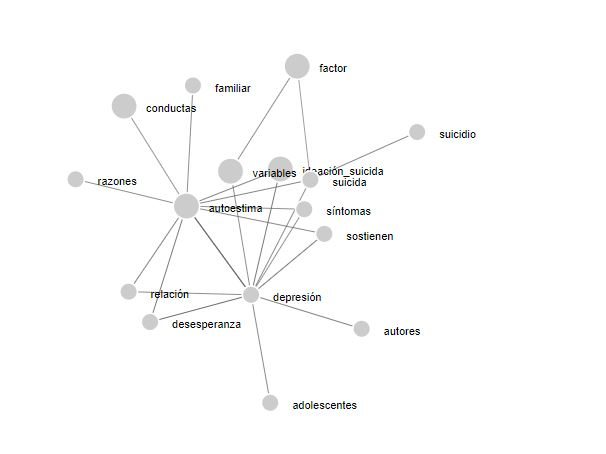
\includegraphics[width=0.8\textwidth]{grupo19}
\caption{Grafo  relaciones temáticas grupo 29 }
\label{fig:grupo19}
\end{figure}

En el grupo 30 se encuentran trabajos relacionados al programa de ingeniería de sistemas, particularmente al área de descubrimiento de conocimiento en base de datos, desarrollo de herramientas bajo el gestor Postgresql, algoritmos de minería de datos, clasificación, agrupación, reglas de asociación y temáticas de software y manejo de información.

\begin{figure}[H]\centering
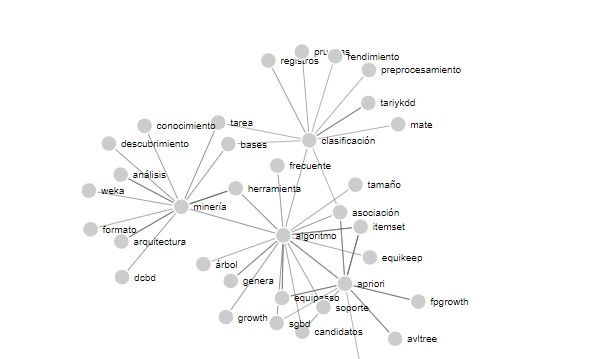
\includegraphics[width=0.8\textwidth]{grafotarykdd}
\caption{Grafo  relaciones temáticas grupo 30 }
\label{fig:tarygradfo}
\end{figure}

En las figuras \ref{fig:tarygradfo}  se muestra el grafo conceptual generado por el modelo Word2vec de los trabajos de grado respectivos al  grupo 30. Donde se pueden establecer vínculos entre conceptos dentro de minería de datos, descubrimiento de conocimiento, algoritmos de clasificación y asociación tales como equipasso, fpgrowth, entrenamiento de  árboles  de decisión, a priori e itemsets frecuentes.

En el grupo 31 se encuentran trabajos de grado relacionados con las ciencias pecuarias, producción acuícola y comparación de dietas en cultivos de peces.



\section{Casos de prueba para trabajos de grado relacionados conceptualmente propuestos por Maskana.}

%Para la evaluación de los trabajos relacionados propuestos por el algoritmo Maskanita \ref{alg:maskanita1}, se realizaron 3 casos de prueba, para los cuales se elaboró una tabla con los resultados obtenidos de las relaciones encontradas para diferentes trabajos de grado, para validar las relaciones propuestas por Maskanita se formaron dos grupos de trabajos; los que fueron relacionados por el algoritmo y los se quedaron por fuera de la frontera de decisión y no se relacionaron, para cada prueba se evalúa el coeficiente de silhouette y se valida la cohesión de los trabajos relacionados y la separación con respecto al grupo de trabajos que no se relacionaron.

Para la evaluación de los trabajos relacionados propuestos por el algoritmo Maskanita \ref{alg:maskanita1}, se realizaron 3 casos de prueba, para los cuales se elaboró una tabla con los resultados obtenidos de las relaciones encontradas para diferentes trabajos de grado.


\begin{table}[H]\centering
\caption{Caso de prueba 1: Resultados recomendación para el trabajo de grado Tariykdd: Una herramienta genérica de descubrimiento de conocimiento en bases de datos débilmente acoplada con el sgbd Postgresql.}\label{tab:tablae1}
	\begin{tabularx}{\textwidth}{XXXm{3.0cm}}\toprule

Id &  \multicolumn{1}{c}{Distancia Milikowski } & \multicolumn{1}{c}{Titulo} \\ 
5268 &0.0006 &Pg\_KDD - Entorno Gráfico para el Sistema de Descubrimiento de 
Conocimiento en Bases de Datos PostgresKDD.   \\ 
446 &  0.0007 &Implantación de primitivas sql para el descubrimiento de reglas de asociación y clasificación al interior del motor del sistema gestor de bases de datos postgresql.   \\ 
183 & 0.0033 &MATE-KDD: Una herramienta genérica para el descubrimiento.   \\ 
4081 &0.0097&EXDACLET: Herramienta de datacleaning basada en agentes inteligentes orientadas a la web \\

 \bottomrule
	\end{tabularx}
	
\end{table}

\begin{table}[H]\centering
\label{tab:tablae1}
	\begin{tabularx}{\textwidth}{XXXm{3.0cm}}\toprule

%Id &  \multicolumn{1}{c}{Distancia Milikowski } & \multicolumn{1}{c}{Titulo} \\ 
4130 & 0.0363  &RASEMUS: Una herramienta para el descubrimiento de conocimiento en bases de datos con técnicas de clustering, débilmente acoplado con el sgbd postgresql. \\ 
6975&0.1320&POLARIS: Herramienta de minería de uso para la web. \\
6206&0.1537&GRFPOSTGRES – Herramienta gráfica para el motor de base de datos postgres.\\
5044&0.1555&STARCUBE: Una herramienta ROLAP de análisis multidimensional para el soporte a la toma de decisiones, débilmente acoplada con el SGBD PostgreSQL. \\
 \bottomrule
	\end{tabularx}
	
\end{table}

%\begin{figure}[H]\centering
%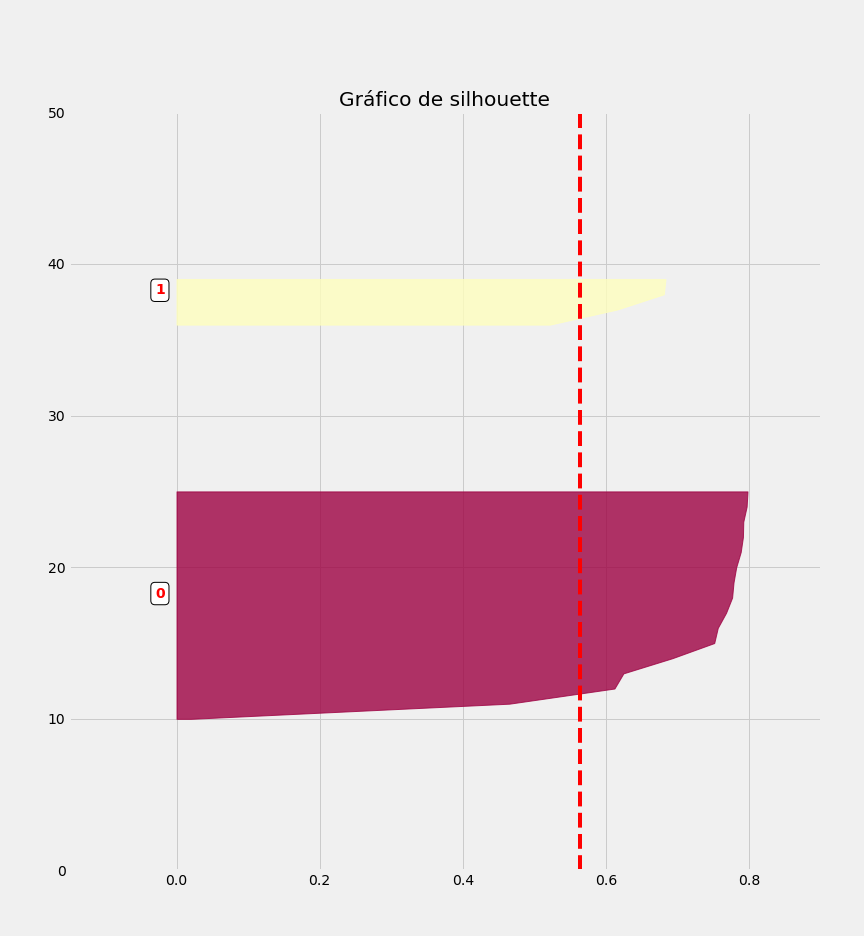
\includegraphics[width=0.8\textwidth]{CoefSil1}
%\caption{Gráfico de Silhouette recomendación caso de prueba 1 }
%\label{fig:silruno}
%\end{figure}




\begin{table}[H]\centering
\caption{Caso de prueba 2: Resultados recomendación para el trabajo de grado Desarrollo e implementación de un sistema de reconocimiento de comandos de voz basado en redes neuronales para la activación de dispositivos electrónicos.}\label{tab:tablae2}
	\begin{tabularx}{\textwidth}{XXXm{3.0cm}}\toprule

Id &  \multicolumn{1}{c}{Distancia Milikowski } & \multicolumn{1}{c}{Titulo} \\ 
5268 &0.0066 &Sistema interactivo de reconocimiento de fonemas para la interpretación de voz y traducción a lengua de señas.  \\ 
446 &  0.0067 &Implementación de redes neuronales artificiales en hardware reconfigurable.Implementación de redes neuronales artificiales en hardware reconfigurable.   \\ 
183 & 0.0087 &Análisis de deformaciones debidas a esfuerzos, vibraciones o variaciones de temperatura en un objeto mediante metrología óptica basada en técnicas de interferometría holográfica.   \\ 
4081 &0.0122&Diseño e implementación de un sistema que activa dispositivos electrónicos mediante señales oculares para mejorar la comunicación a personas con discapacidad motora. \\
4130 & 0.0314  &Detección automática de registros sísmicos asociados al comportamiento del volcán galeras haciendo uso de redes. \\ 

 \bottomrule
	\end{tabularx}
	
\end{table}


\begin{table}[H]\centering
\label{tab:tablae2}
	\begin{tabularx}{\textwidth}{XXXm{3.0cm}}\toprule

%Id &  \multicolumn{1}{c}{Distancia Milikowski } & \multicolumn{1}{c}{Titulo} \\ 
6975&0.0395&Evaluar un acople colimador fibra óptica para valorar su comportamiento como medidor de intensidad luminosa. \\
6206&0.0476&Optimización de un sistema de control para la navegación basado en el método de campo de fuerza virtual para un vehículo autónomo empleando algoritmos genéticos.\\
5044&0.0526&Diseño e implementación de un sistema portátil de registro de señales micro-sísmicas. \\
5044&0.0648&Identificación de aves a partir de canto característico e información contenida en bases de datos. \\
5044&0.0786&Diseño e implementación del prototipo de un osciloscopio. \\

 \bottomrule
	\end{tabularx}
	
\end{table}

%\begin{figure}[H]\centering
%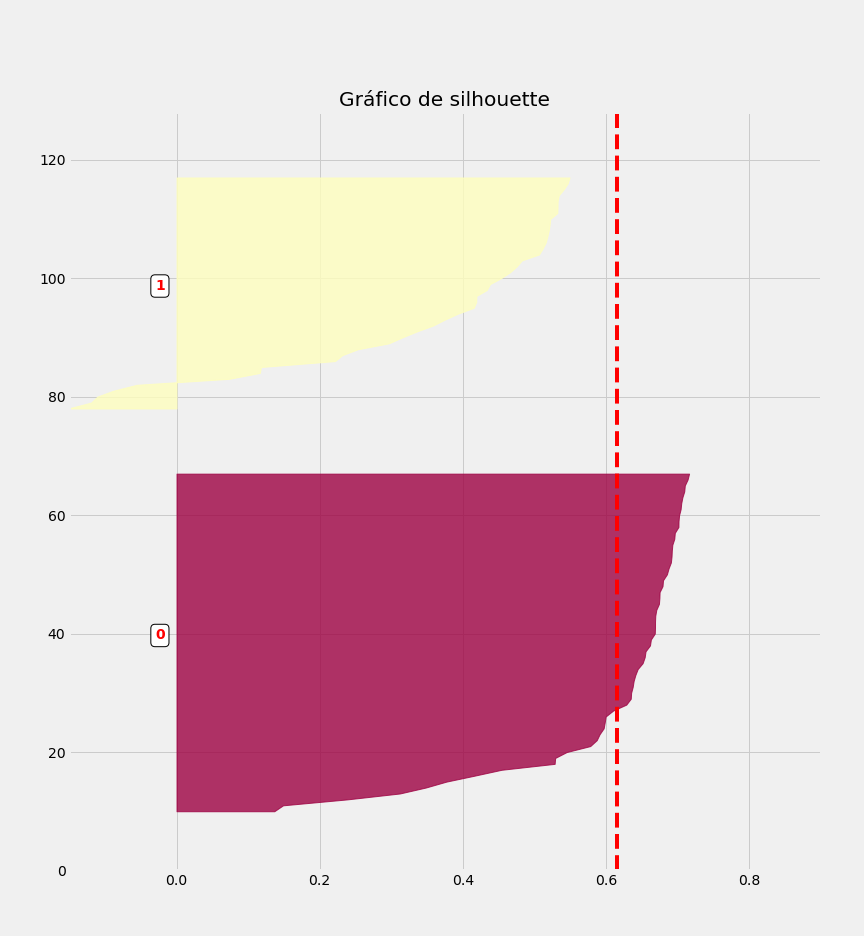
\includegraphics[width=0.8\textwidth]{CoefSil2}
%\caption{Gráfico de Silhouette recomendación caso de prueba 2 }
%\label{fig:silrdos}
%\end{figure}

\begin{table}[H]\centering
\caption{Caso de prueba 3: Resultados recomendación para el trabajo de grado Construcción de un repositorio limpio de datos para la detección de patrones de eventos eruptivos del volcán galeras con técnicas de minería de datos.}\label{tab:tablae3}
	\begin{tabularx}{\textwidth}{XXXm{3.0cm}}\toprule

Id &  \multicolumn{1}{c}{Distancia Milikowski } & \multicolumn{1}{c}{Titulo} \\ 
5268 &0.0685 &Detección automática de registros sísmicos asociados al comportamiento del volcán galeras haciendo uso de redes neuronales artificiales.  \\ 
446 & 0.1015 &Monitoreo electromagnético de volcanes.   \\ 
183 & 0.1615 &Implementación de un método fundamentado en la distribución de amplitudes para la localización de sismos asociados al movimiento de fluidos en el volcán galeras, Colombia.   \\ 
4081 &0.3012&Diseño e implementación de estación modelo de registro, trasmisión y recepción de eventos micro-sísmicos de la red sísmica de san juan de pasto. \\
4130 & 0.3286&Diseño e implementación del prototipo de una estación meteorológica automática portátil capaz de transmitir los datos mediante tecnología gsm. \\ 

 \bottomrule
	\end{tabularx}
	
\end{table}

%\begin{figure}[H]\centering
%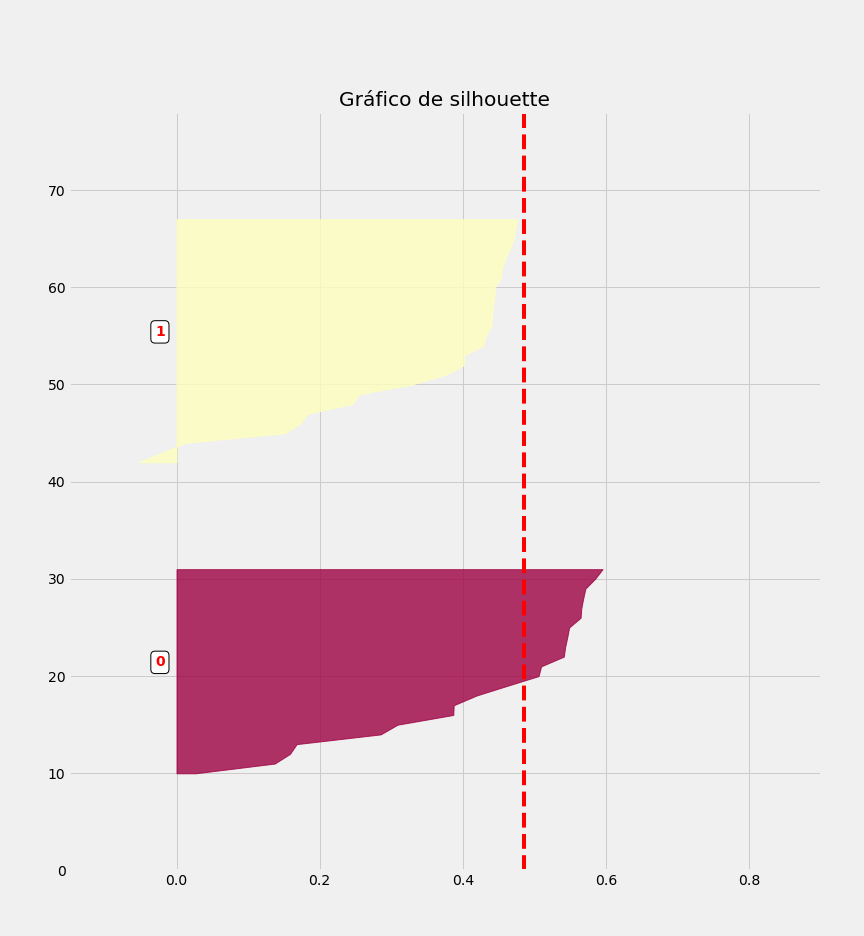
\includegraphics[width=0.8\textwidth]{CoefSil3}
%\caption{Gráfico de Silhouette recomendación caso de prueba 3 }
%\label{fig:silrtres}
%\end{figure}


%En las figura \ref{fig:silruno}, \ref{fig:silrdos} y ~\ref{fig:silrtres} se puede apreciar que los documentos relacionados propuestos por Maskanita (color rojo) están cohesionados de forma correcta a su grupo, ya que no se observan valores de silueta negativos, los valores promedio de silhouette para los 3 casos son de 0.58, 0.62 y 0.5 respectivamente; indicando  que los grupos se ajustan adecuadamente, en las ~\ref{fig:silrdos} y  ~\ref{fig:silrtres} se puede observar algunos valores de silhouette negativos en el grupo de documentos que no fueron relacionados por Maskanita (color amarillo), lo cual indica que no se cohesionan correctamente, ya que podría existir un tercer grupo o tercer dominio donde estos se agrupen adecuadamente; lo cual no es de importancia ya que la atención se centra en el grupo de documentos relacionados por el método implementado.






